\subsection{Fuzzy következtető módszer, defuzzifikációs módszerek.}

\textbf{Fuzzy rendszer általános sémája:}
\begin{center}
    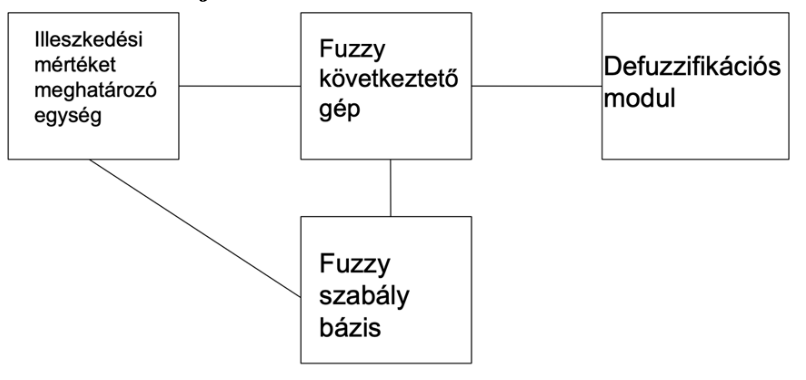
\includegraphics[width=0.7\textwidth]{res/imgs/info_17_schema.png}
\end{center}

\textbf{Fuzzy szabályozás -- példa:}
\begin{center}
    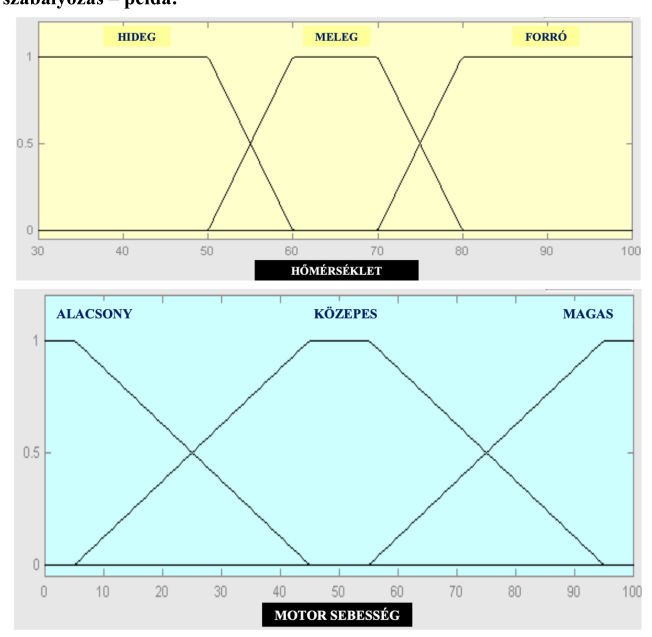
\includegraphics[width=0.6\textwidth]{res/imgs/info_17_rules.png}
\end{center}

\begin{enumerate}
    \item \textbf{Ha} a \textit{hőmérséklet} HIDEG \textbf{akkor} a \textit{motor sebesség} ALACSONY
    \item \textbf{Ha} a \textit{hőmérséklet} MELEG \textbf{akkor} a \textit{motor sebesség} KÖZEPES
    \item \textbf{Ha} a \textit{hőmérséklet} FORRÓ \textbf{akkor} a \textit{motor sebesség} MAGAS
\end{enumerate}

\begin{itemize}
    \item A a szabály antecedense, B pedig a konzekvense
\end{itemize}

\textbf{Fuzzy következtető módszer:}
\begin{itemize}
    \item a következtetéshez szükségünk van a fuzzy-szabályok s normájára (unió) „szabálybázis”
    \item megállapítjuk a konkrét bemeneti értékeknél az antecedens tagsági függvény (illeszkedési) értékeit a bemeneti partícióban
    \item az illeszkedési értékekkel levágjuk a konzekvens partíció függvényeit
    \item ezek s-normáját (unióját) vesszük
    \item a defuzzifikációs modul egy konkrét értéket szolgáltat, valamely módszerrel:
    \begin{itemize}
        \item súlyponti módszer
        \item összegek közepe módszer
        \item középső maximum módszer
    \end{itemize}
\end{itemize}

\textbf{Súlyponti módszer:}
\begin{itemize}
    \item S norma
\end{itemize}
\begin{center}
    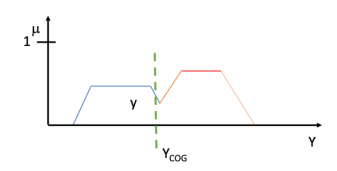
\includegraphics[width=0.5\textwidth]{res/imgs/info_17_cog.png}
\end{center}
\begin{itemize}
    \item $Y_{COG} = \frac{\int_{y \in Y} y \mu_y(y) dy}{\int_{y \in Y} \mu_y(y) dy}$
\end{itemize}

\textbf{Összegek közepe módszer:}
\begin{itemize}
    \item S norma
\end{itemize}
\begin{center}
    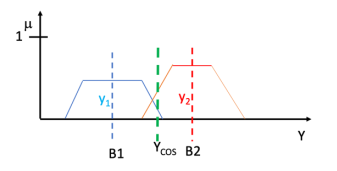
\includegraphics[width=0.5\textwidth]{res/imgs/info_17_cos.png}
\end{center}
\begin{itemize}
    \item $Y_{COS} = \frac{\sum_{i=1}^r y_i \int_{y \in Y} y \mu_{y_i}(y) dy}{\sum_{i=1}^r \int_{y \in Y} \mu_{y_i}(y) dy}$
\end{itemize}

\textbf{Középső maximum módszer:}
\begin{itemize}
    \item S norma
\end{itemize}
\begin{center}
    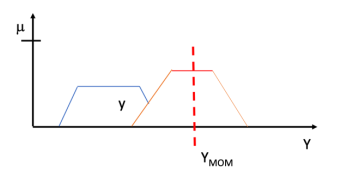
\includegraphics[width=0.5\textwidth]{res/imgs/info_17_mom.png}
\end{center}
\begin{itemize}
    \item $Y_{MOM} = \frac{\int_{y \in MAX(\mu_Y)} y dy}{\int_{y \in MAX(\mu_Y)} dy}$
\end{itemize}

\textbf{Következtető módszer példa:}
\begin{center}
    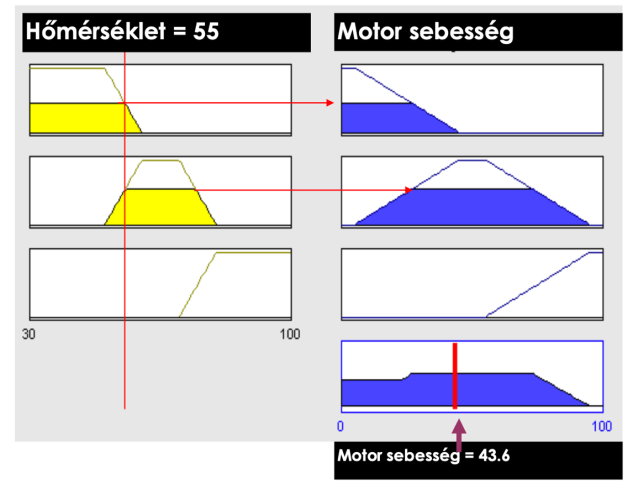
\includegraphics[width=0.6\textwidth]{res/imgs/info_17_example.png}
\end{center}